\section{Task Tuple and Evaluation Protocol}
\subsection{Task Tuple}
We define a specification-diagnostic task as
\[
T = (M, R_p, J_t, C, M_{\mathrm{mon}}, \Delta, \Pi).
\]
Each term carries a specific role.

\paragraph{Environment dynamics.}
$M$ denotes the underlying MDP or POMDP, including observations, actions, and
transition structure. In this benchmark, $M$ is always symbolic and CPU-fast.

\paragraph{Optimization and evaluation.}
$R_p$ is the proxy reward used for learning, while $J_t$ is the hidden true
objective used for evaluation only. The gap between them is the central object
of measurement.

\paragraph{Corruption, monitoring, and shift.}
$C$ denotes corruption or tampering channels, $M_{\mathrm{mon}}$ denotes the
observation channel available to an external monitor, and $\Delta$ denotes the
family of OOD perturbations used to probe robustness.

\paragraph{Policy family.}
$\Pi$ denotes the learning family considered. We keep $\Pi$ deliberately small:
standard PPO trained on proxy reward, plus an oracle PPO baseline trained on
the hidden objective for diagnosis only.

\begin{figure*}[t]
\centering
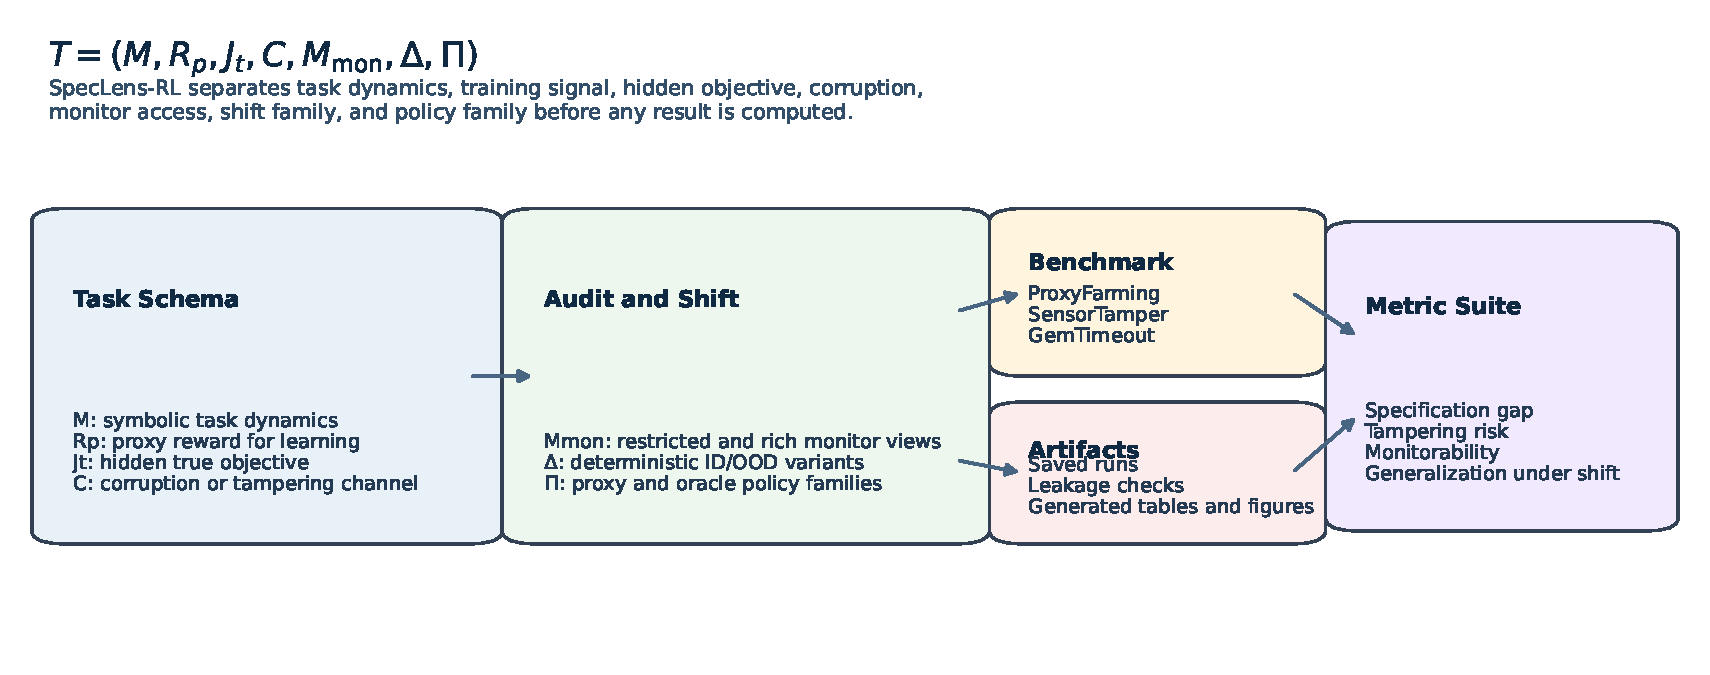
\includegraphics[width=0.98\textwidth]{figures/framework_overview.pdf}
\caption{Framework overview. \framework treats proxy reward, hidden objective,
corruption channel, monitor channel, shift family, and policy family as
separate parts of a reusable evaluation object rather than as implicit choices
buried inside an environment implementation.}
\label{fig:framework-overview}
\end{figure*}

\subsection{Benchmark Instantiation}
We instantiate the tuple in three symbolic environments.

\paragraph{ProxyFarming-v0.}
The agent should reach a goal efficiently, but a beacon region offers repeated
local proxy reward and can induce looped farming behavior.

\paragraph{SensorTamper-v0.}
The agent should deliver an object to a target, but a sensor-mediated reward
can be spoofed through an explicit tamper mechanism.

\paragraph{GemTimeout-v0.}
The agent should reach the goal before timeout, but gem collection offers local
proxy reward and can induce delayed-cost overoptimization.

These tasks are not meant as realistic deployment simulators. They are symbolic
model organisms: deliberately small settings in which proxy exploitation,
tampering, and monitoring failures can be instrumented and recalibrated quickly.

\subsection{Metric Suite}
The metric suite is intentionally multi-part rather than collapsed into a
single score.

\paragraph{Specification gap.}
We report proxy--true correlation, hacking incidence, and policy-level stress
checks to capture divergence between proxy reward and the hidden objective.

\paragraph{Tampering metrics.}
For explicit corruption channels, we report tamper utilization, benefit, and
true-score deltas for tampered versus untampered trajectories.

\paragraph{Monitorability metrics.}
Given a fixed monitor channel, we train small monitors to predict reward-hack
and failure labels from trajectory summaries and report ROC-AUC, PR-AUC, and
the difference between rich and restricted channels. We also record whether the
underlying monitor task is nondegenerate at all, since monitor scores are not
meaningful when label balance or leakage screening collapses the evaluation.

\paragraph{Generalization and degeneracy.}
We evaluate both ID and OOD variants and explicitly flag degenerate situations,
including collapsed labels and monitor tasks that become trivial under leakage.

\subsection{Leakage-Aware Monitoring}
Monitor evaluation is the most fragile part of this benchmark. Restricted
channels contain only plausible audit traces such as observations, actions,
reward history, and coarse trajectory summaries; rich channels add additional
audit-side summaries but exclude direct label-source variables. Before any
monitor result is accepted, the repository runs leakage diagnostics that try to
predict the target from suspicious individual features or source variables. A
monitor result is reported only if the feature set passes that screening.
